% *****************************************************************************
%
%        CNB OAM Document Classifier - Research Report
%        Faculty of Applied Sciences, University of West Bohemia
%
%        Encoding: UTF-8
%        TeXer:    pdflatex
%
% *****************************************************************************

\documentclass[czech, oth, kky, he, iso690alph, pdf, viewonly]{fasthesis}%
\title{Klasifikace a validace dokumentů regulovaných informací ČNB OAM}
\worktypespec{Výzkumná zpráva}
\author{Student}{ZČU}{}{}
\supervisor{doc. Ing. Kamil Ekštein, Ph.D.}
\stagworkid{99999}
\signdate{30}{5}{2026}{V Plzni}

\addbibresource{manual.bib}

\abstract{Tato výzkumná zpráva se zabývá problematikou automatické klasifikace a validace dokumentů odesílaných do portálu regulovaných informací České národní banky (ČNB OAM) \cite{cnboam}. Cílem projektu je vytvořit robustní softwarový systém pro sběr dat z portálu ČNB OAM a vyhodnotit úspěšnost různých metod strojového učení a velkých jazykových modelů (LLM) při klasifikaci těchto dokumentů do příslušných kategorií. V práci je popisán návrh a implementace webového škrabáku (scraperu) s využitím knihovny Playwright \cite{playwright}, metodika předzpracování textu a následné experimenty s pravidlovými systémy, tradičními modely (TF-IDF ve spojení s logistickou regresí, náhodnými lesy a SVM) a velkým jazykovým modelem Gemma 3 (12B) běžícím na univerzitním serveru s Digest autentizací. Výsledky ukazují, že nejvyšší celkové přesnosti dosahuje lineární SVM (95,0~\%), což výrazně překonává model Gemma 3 v zero-shot režimu (66,2~\%) i pravidlovou baseline (72,2~\%).}{This research report addresses the automated classification and validation of regulatory documents submitted to the Czech National Bank's OAM portal \cite{cnboam}. The objective of this project is to build a robust data collection pipeline and evaluate the performance of various machine learning and large language model (LLM) approaches in classifying these documents. We describe the design and implementation of a custom scraper using the Playwright library \cite{playwright}, text preprocessing techniques, and subsequent experiments with rule-based systems, traditional ML classifiers (TF-IDF combined with Logistic Regression, Random Forest, and Linear SVM), and the Gemma 3 (12B) LLM running on the university server. The evaluation results show that the Linear SVM achieves the highest accuracy (95.0\%), significantly outperforming the zero-shot Gemma 3 LLM (66.2\%) and the rule-based baseline (72.2\%).}

\keywords{klasifikace textu, Česká národní banka, ČNB OAM, strojové učení, TF-IDF, SVM, velký jazykový model, Gemma 3}

\acknowledgement{Rád bych na tomto místě poděkoval za poskytnutí přístupu k výpočetnímu serveru Ollama s modelem Gemma 3 a za podporu při realizaci tohoto projektu.}

\begin{document}
\frontpages[notm]
\tableofcontents

% _____________________________________________________________________________
%        KAPITOLA 1: Úvod
% _____________________________________________________________________________
\chapter{Úvod}
Portál oficiálního úložiště regulovaných informací České národní banky (ČNB OAM) slouží k uveřejňování zákonem předepsaných informací emitenty cenných papírů. Emitenti jsou povinni odesílat různé typy dokumentů, jako jsou výroční finanční zprávy, pololetní finanční zprávy, vnitřní informace, pozvánky na valné hromady a další. 

V praxi však dochází k situacím, kdy emitenti odesílají nesprávné typy dokumentů nebo dokumenty neodpovídající deklarované kategorii. Ruční kontrola každého vloženého dokumentu a jeho příloh je časově i personálně velmi náročná. Z tohoto důvodu vzniká potřeba automatizovaného systému, který by dokázal analýzovat textový obsah odeslaných příloh a validovat, zda odpovídá deklarovanému typu informace.

Tento projekt se zaměřuje na vytvoření kompletního řešení, které zahrnuje:
\begin{enumerate}
    \item Automatizovaný sběr dat (scraping) z portálu ČNB OAM, stahování příloh a extrakci textu.
    \item Návrh a trénování klasifikačních modelů pro rozřazování dokumentů do 12 aktivních kategorií.
    \item Nasazení velkého jazykového modelu (Gemma 3) prostřednictvím univerzitního serveru Ollama jako zero-shot/few-shot klasifikátoru.
    \item Validaci shody mezi deklarovanou kategorií dokumentu a jeho skutečným obsahem.
\end{enumerate}

V dalších kapitolách je popsáno teoretické pozadí klasifikace textu, praktické detaily naší implementace a dosažené výsledky srovnání jednotlivých modelů.

% _____________________________________________________________________________
%        KAPITOLA 2: Teoretické zázemí
% _____________________________________________________________________________
\chapter{Teoretické zázemí}
Klasifikace textu je standardní úlohou zpracování přirozeného jazyka (NLP). V tomto projektu porovnáváme pět různých přístupů.

\section{Pravidlový systém (Rule-based)}
Pravidlový klasifikátor představuje základní baseline řešení. Funguje na principu vyhledávání klíčových slov a regulárních výrazů v textu dokumentu. Pro každou kategorii je definována sada charakteristických českých a anglických termínů (např. „valná hromada“ pro pozvánky, „výroční zpráva“ pro výroční zprávy). Dokument je zařazen do té kategorie, která získá nejvyšší skóre na základě frekvence výskytu těchto termínů. Tento přístup je velmi rychlý a deterministický, ale špatně se adaptuje na jazykovou variabilitu a chybějící synonyma.

\section{TF-IDF vektorizace}
TF-IDF (\textsl{Term Frequency-Inverse Document Frequency}) je statistická míra vyjadřující důležitost slova pro daný dokument v rámci celého korpusu \cite{salton1988term}. Vektorizace převádí texty na numerické vektory, kde každá dimenze reprezentuje jedno slovo (či n-gram) a hodnota odpovídá jeho TF-IDF skóre.
Formule pro TF-IDF je:
\begin{equation}
    \text{TF-IDF}(t, d, D) = \text{TF}(t, d) \times \text{IDF}(t, D)
\end{equation}
kde $\text{TF}(t, d)$ je relativní frekvence termínu $t$ v dokumentu $d$ a $\text{IDF}(t, D) = \log \frac{|D|}{1 + |\{d \in D : t \in d\}|}$ je inverzní frekvence dokumentu v korpusu $D$.

Na tyto vektory jsou následně aplikovány klasické algoritmy strojového učení implementované pomocí knihovny Scikit-learn \cite{scikit-learn}:
\begin{itemize}
    \item \textbf{Logistická regrese}: Lineární model, který odhaduje pravděpodobnosti tříd pomocí logistické funkce.
    \item \textbf{Náhodný les (Random Forest)}: Ansámblová metoda založená na rozhodovacích stromech, která snižuje riziko přetrénování průměrováním predikcí jednotlivých stromů.
    \item \textbf{Support Vector Machines (SVM)}: Hledá optimální nadrovinu, která maximalizuje marži mezi třídami. Lineární SVM je pro klasifikaci textu vysoce efektivní kvůli vysoké dimenzionalitě textových vektorů \cite{cortes1995support}.
\end{itemize}

\section{Velké jazykové modely (LLM)}
Velké jazykové modely založené na architektuře Transformer (např. řada Gemma od společnosti Google \cite{gemma3}) dosahují vynikajících výsledků v úlohách porozumění textu. V naší práci využíváme model \textbf{Gemma 3 (12B)} běžící na univerzitním Ollama serveru. 

Tento model je dotazován pomocí strukturovaného promptu v češtině, který specifikuje dostupné kategorie a pravidla pro zařazení. Model je instruován, aby odpověděl výhradně ve formátu JSON obsahujícím klíče \texttt{category} a \texttt{reason} (odůvodnění predikce). Používáme zero-shot (bez příkladů) nebo few-shot (s několika málo příklady v promptu) přístup. Tím odpadá nutnost trénování parametrů modelu na lokálním hardwaru, což je ideální pro nasazení bez dedikovaných grafických karet (GPU).

% _____________________________________________________________________________
%        KAPITOLA 3: Praktická implementace
% _____________________________________________________________________________
\chapter{Praktická implementace}
Softwarový systém je napsán v jazyce Python 3 a skládá se ze tří hlavních modulů: scraperu, předzpracování textu a klasifikátoru.

\section{Sběr dat (Scraping)}
Portál ČNB OAM \cite{cnboam} je postaven na technologii Oracle BI Publisher, která dynamicky generuje stránky a využívá vnitřní iframy pro tabulky výsledků. Původní implementace s běžnou navigací přes tlačítko „Další výsledky“ trpěla zasekáváním v headless režimu prohlížeče Chromium, kdy portál otevíral nová okna bez přenosu session cookie a vracel prázdný loading.jsp.

Tento problém jsme vyřešili robustním hybridním přístupem. Scraper se nejprve pokouší o přímou navigaci na odkaz „Další výsledky“ (s parametrem \texttt{par\_count=C1A}), který zobrazí celou historii najednou na jedné stránce. Pokud tento pokus z důvodu velkého objemu dat nebo pomalé odezvy serveru selže, systém automaticky přejde na záložní režim krájení dotazů po jednotlivých letech (date-range slicing), což zajišťuje vysokou stabilitu stahování. Detaily dokumentů jsou následně parsovány z dynamického iframu \texttt{xdo:docframe0} pomocí knihovny Playwright \cite{playwright}.

\section{Předzpracování textu (Head-Tail Truncation)}
Klasifikované dokumenty (často PDF soubory, naskenované dokumenty převedené přes OCR nebo ZIP archivy) mohou být extrémně dlouhé (stovky stran). Většina klíčových informací o kategorii (jako je název dokumentu, např. „Výroční zpráva“, „Pozvánka...“) se nachází na první straně (hlavička) nebo na samotném konci (podpisy a schválení). 

Pro snížení šumu a splnění limitu kontextového okna transformerů (512 tokenů u standardního BERTU nebo omezení promptu u LLM) jsme implementovali metodu **ořezávání hlavy a paty (head-tail truncation)**. Pokud text dokumentu překročí 20~000 znaků, zachováme prvních 15~000 znaků a posledních 5~000 znaků a prostřední část textu zahodíme. Tento krok výrazně zlepšil přesnost a rychlost trénování.

\section{Integrace s Ollama API}
Modul \texttt{OllamaLLMClassifier} zajišťuje komunikaci s výpočetním serverem přes REST API. Vzhledem k tomu, že server vyžaduje zabezpečený přístup, implementovali jsme podporu pro **Digest autentizaci** pomocí knihovny \texttt{httpx.DigestAuth}. Klient nejprve zachytí výzvu \texttt{401 Unauthorized}, získá jednorázový nonce a následně odešle hashovaný požadavek, který server schválí a vrátí predikovaný JSON.

% _____________________________________________________________________________
%        KAPITOLA 4: Výsledky srovnání
% _____________________________________________________________________________
\chapter{Výsledky srovnání}
V této kapitole uvádíme výsledky srovnání všech pěti klasifikačních metod na expandovaném datasetu regulovaných informací ČNB OAM.

\section{Dataset a experimentální nastavení}
Dataset byl rozšířen a data byla rozdělena na trénovací split (70~\%), validační split (10~\%) a testovací split (20~\%) z celkového počtu 4~284 vyfiltrovaných dokumentů. Podrobné rozdělení velikostí jednotlivých splitů je uvedeno v tabulce~\ref{tab:splits}. Vyhodnocení proběhlo na testovacím splitu pomocí metriky přesnosti (Accuracy), Macro F1-skóre a váženého F1-skóre (Weighted F1).

\begin{table}[h]
\centering
\caption{Rozdělení datasetu do jednotlivých splitů}
\label{tab:splits}
\begin{tabular}{lrr}
\hline
Split & Počet dokumentů & Procento \\
\hline
Trénovací (Train) & 2~998 & 70,0~\% \\
Validační (Val) & 429 & 10,0~\% \\
Testovací (Test) & 857 & 20,0~\% \\
\hline
Celkem & 4~284 & 100,0~\% \\
\hline
\end{tabular}
\end{table}

\section{Celkové výsledky srovnání}
V tabulce~\ref{tab:results} je uvedeno celkové srovnání úspěšnosti jednotlivých modelů.

\begin{table}[h]
\centering
\caption{Celkové srovnání klasifikačních metod na testovacím splitu}
\label{tab:results}
\begin{tabular}{lrrr}
\hline
Metoda & Přesnost (Accuracy) & Macro F1 & Weighted F1 \\
\hline
Rule-based (Pravidla) & 0.722 & 0.488 & 0.724 \\
TF-IDF + Logistická regrese & 0.898 & 0.760 & 0.908 \\
TF-IDF + Náhodný les (RF) & 0.933 & 0.734 & 0.930 \\
Ollama LLM (Gemma 3 12B) & 0.662 & 0.520 & 0.678 \\
\textbf{TF-IDF + SVM (Linear)} & \textbf{0.950} & \textbf{0.788} & \textbf{0.949} \\
\hline
\end{tabular}
\end{table}

Z výsledků vyplývá, že **nejlepšího výkonu** dosáhl model **TF-IDF + SVM (Linear)** s celkovou přesností \textbf{94,98~\%} a Weighted F1 skórem \textbf{94,86~\%}. Tento model těží z robustního vyhledávání oddělující nadroviny ve vysokodimenzionálním prostoru slovních n-gramů a vykazuje výborné vlastnosti i při klasifikaci méně zastoupených tříd.

Tradiční klasifikátory trénované s dohledem (supervised), jako je logistická regrese (přesnost 89,85~\%) a náhodné lesy (přesnost 93,35~\%), dosahují na tomto větším datasetu vynikajících výsledků a výrazně překonávají pravidlovou baseline (přesnost 72,23~\%). 

Naopak model **Ollama LLM (Gemma 3 12B)** v režimu zero-shot vykazuje na celých 12 třídách nižší přesnost (**66,18~\%**). Tento pokles je způsoben vysokou sémantickou podobností dokumentů v některých kategoriích (např. pozvánky na valné hromady versus usnesení z valných hromad), kde zero-shot promptování bez předchozího trénování na doménových datech nedokáže spolehlivě rozlišit jemné právní a časové rozdíly v českých textech, což vede k záměnám. Supervised modely (zejména SVM) se tyto jemné rozdíly naučily na trénovacích datech rozlišovat mnohem lépe.

\section{Detailní analýza a vizualizace}
Pro detailní analýzu chyb jsou k dispozici matice záměn (\textsl{confusion matrix}) a grafy F1-skóre pro jednotlivé třídy. Tyto výstupy byly uloženy do adresáře výsledků a jsou automaticky generovány vyhodnocovací sadou.

Na obrázku~\ref{fig:method_comparison} je zobrazeno celkové srovnání přesnosti (Accuracy) a F1-skóre (Macro i Weighted) pro všech pět zkoumaných metod. Je patrné, že tradiční klasifikátory s dohledem dosahují lepších a vyrovnanějších výsledků než zero-shot LLM či pravidlový systém.

\begin{figure}[htbp]
    \centering
    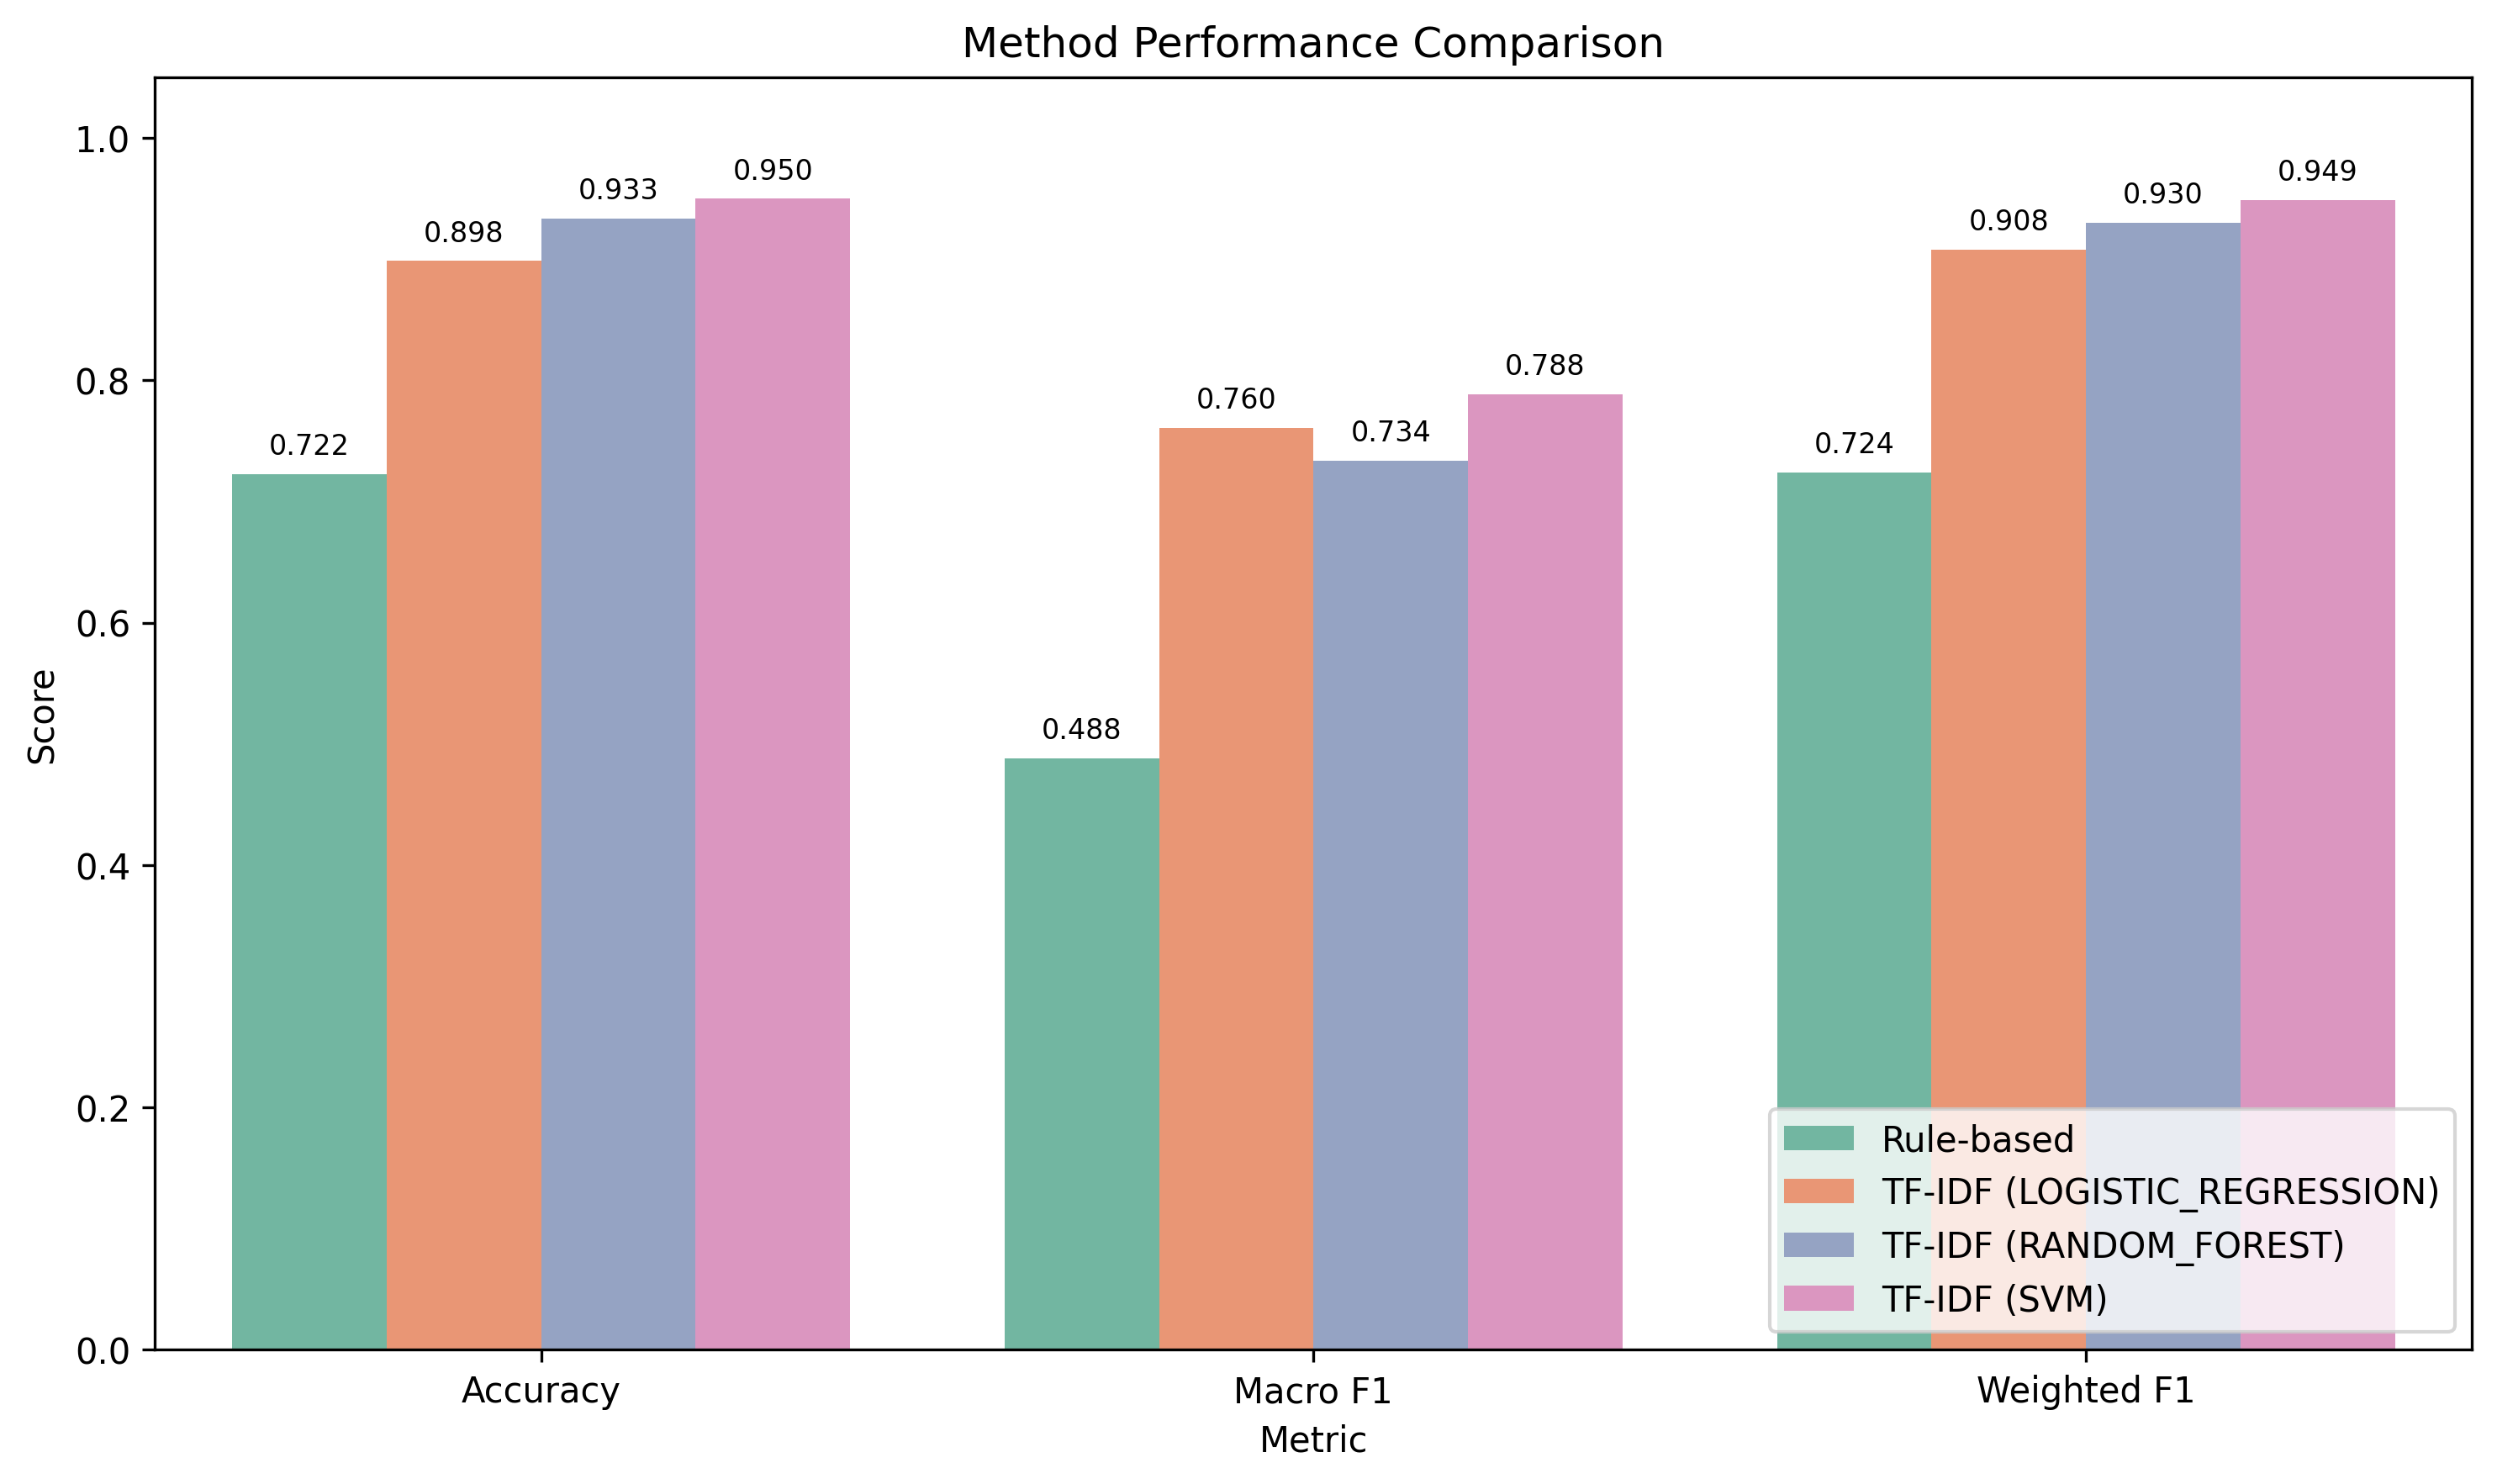
\includegraphics[width=0.85\textwidth]{img/method_comparison.png}
    \caption{Celkové srovnání přesnosti a F1-skóre jednotlivých modelů}
    \label{fig:method_comparison}
\end{figure}

Obrázek~\ref{fig:f1_comparison} ukazuje detailní srovnání F1-skóre pro jednotlivé třídy napříč všemi modely. Zde je vidět, že třídy s nízkým zastoupením v testovacích datech (např. výroční zprávy s nízkým recall) vykazují větší kolísání.

\begin{figure}[htbp]
    \centering
    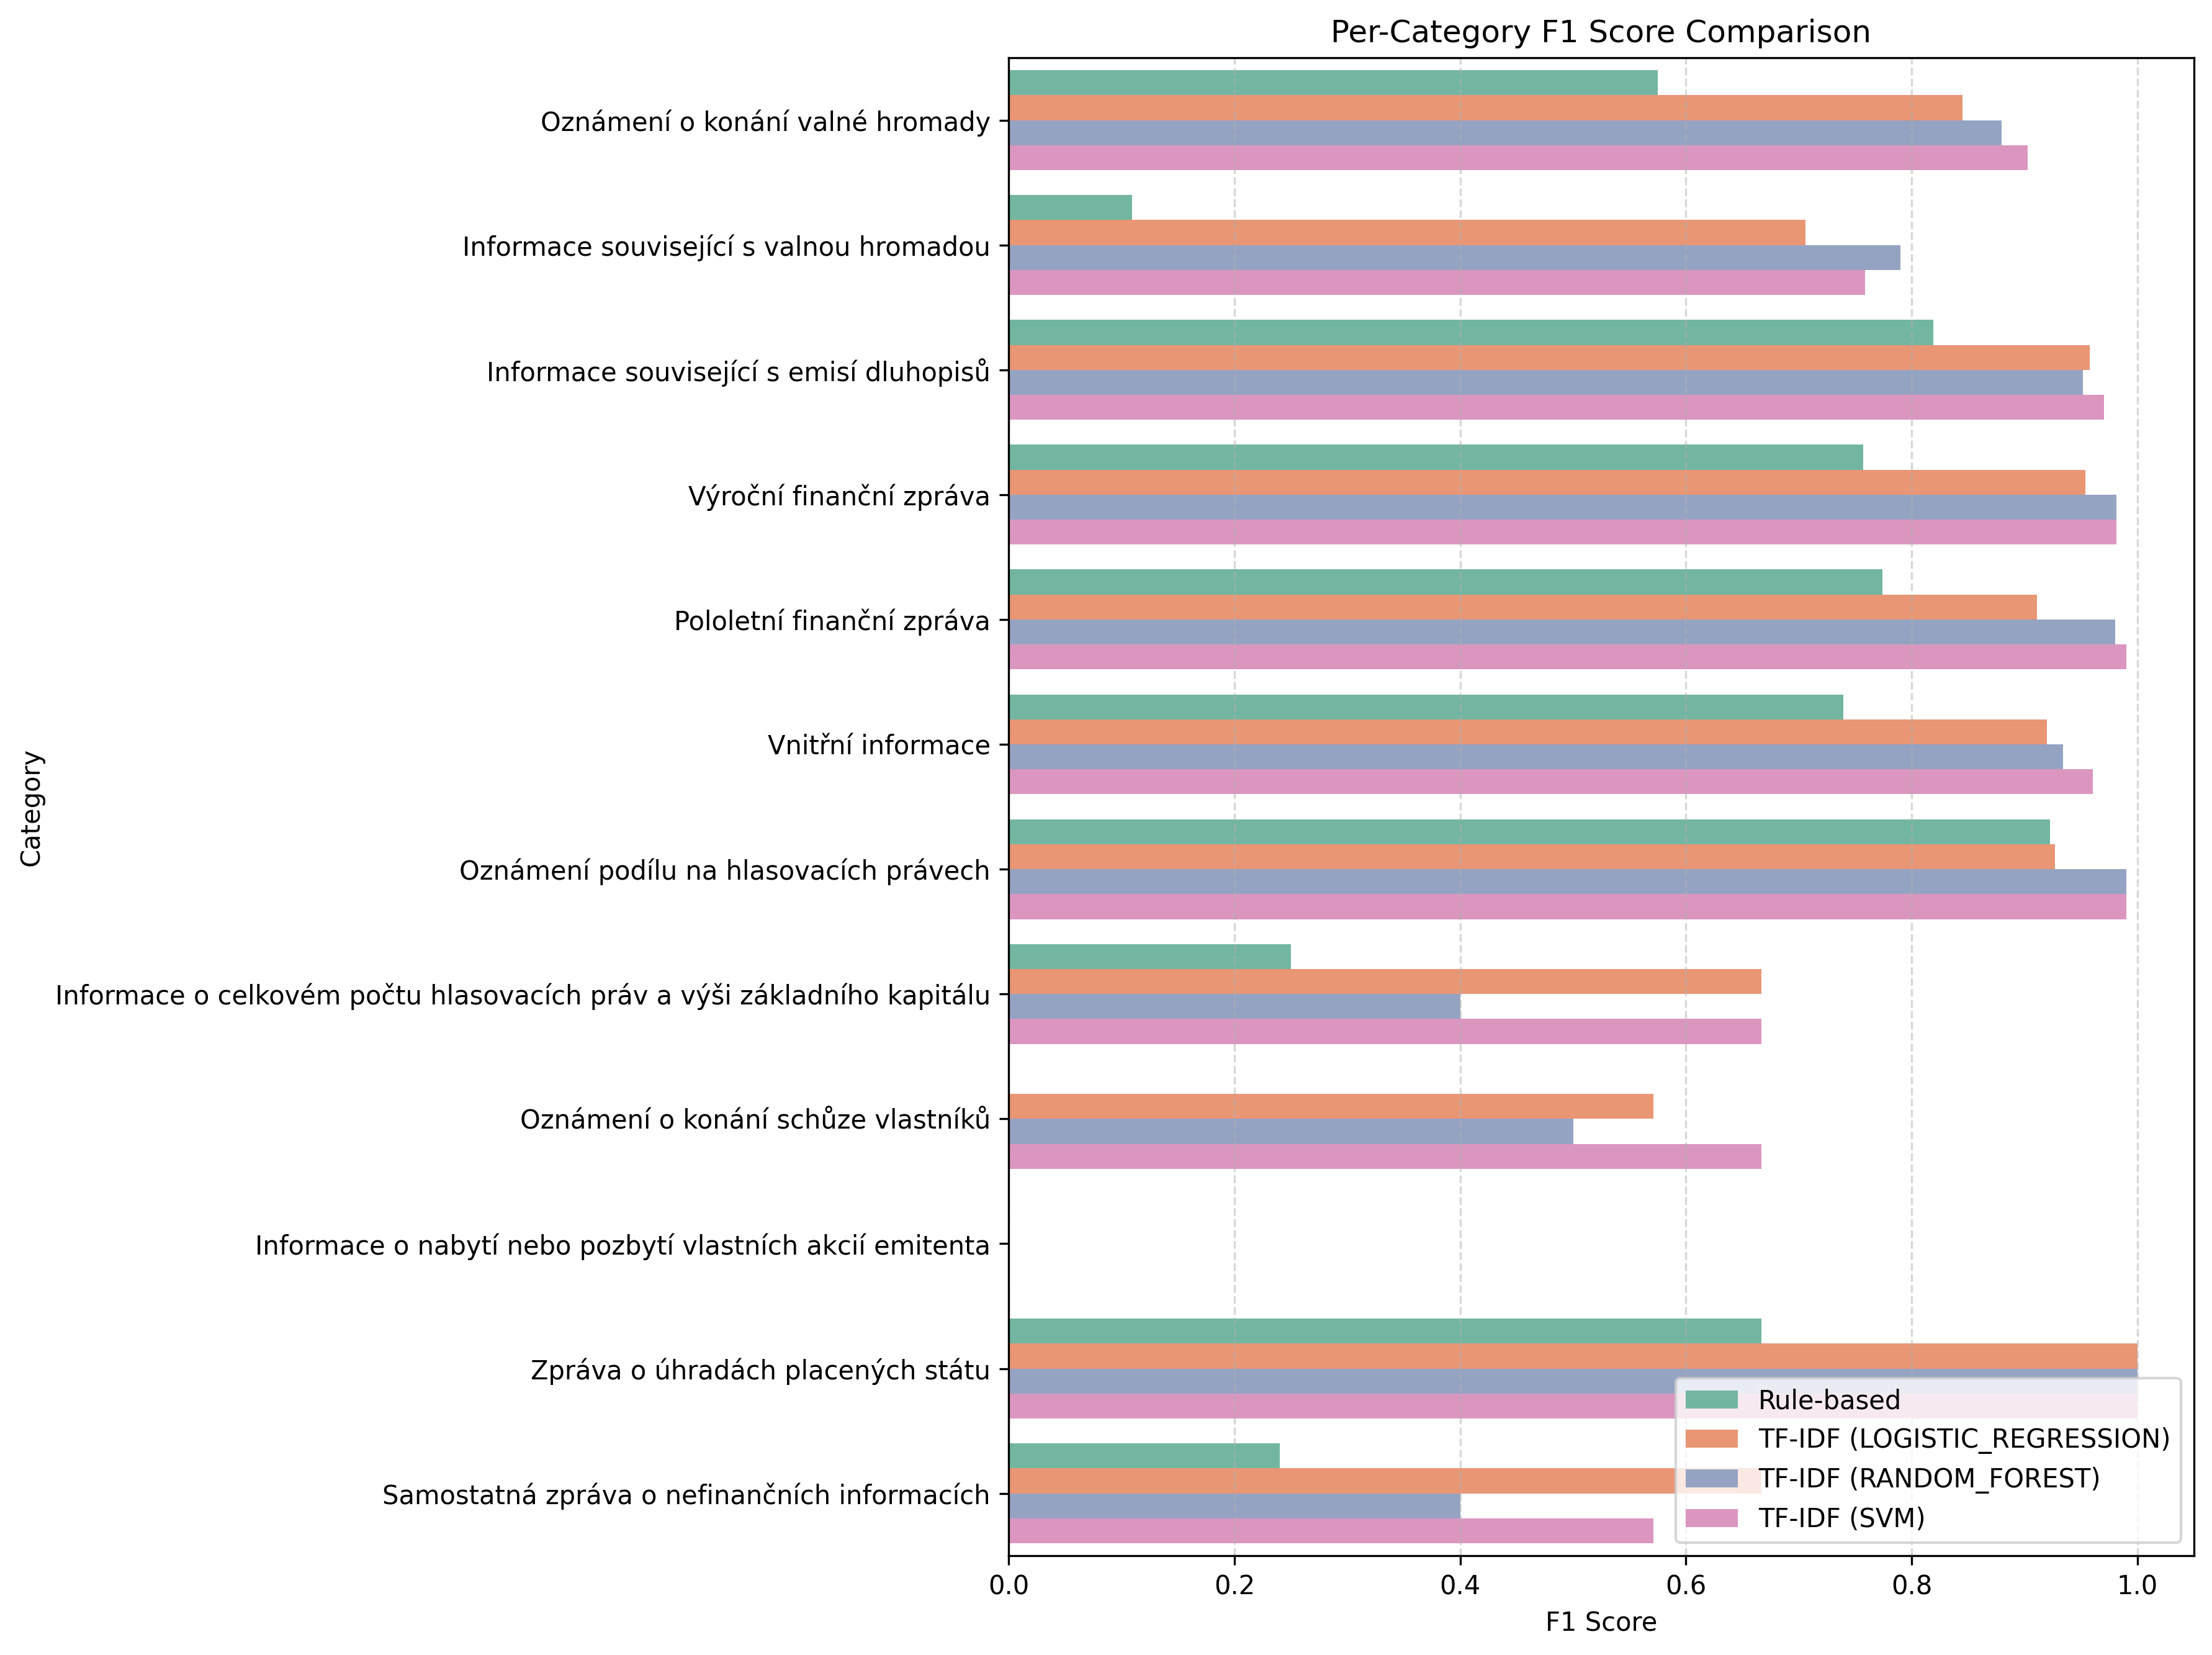
\includegraphics[width=0.85\textwidth]{img/per_class_f1_comparison.png}
    \caption{Porovnání F1-skóre pro jednotlivé kategorie dokumentů}
    \label{fig:f1_comparison}
\end{figure}

Obrázek~\ref{fig:confusion_svm} znázorňuje matici záměn pro nejlepší model, tedy lineární SVM. 
Z analýzy matice záměn vyplývá, že k nejčastějším chybám dochází mezi kategoriemi „Oznámení o konání valné hromady“ a „Informace související s valnou hromadou“, což je logické, neboť oba typy dokumentů sdílejí téměř totožný slovník a často se vyskytují v rámci jednoho PDF souboru odeslaného emitentem.

\begin{figure}[htbp]
    \centering
    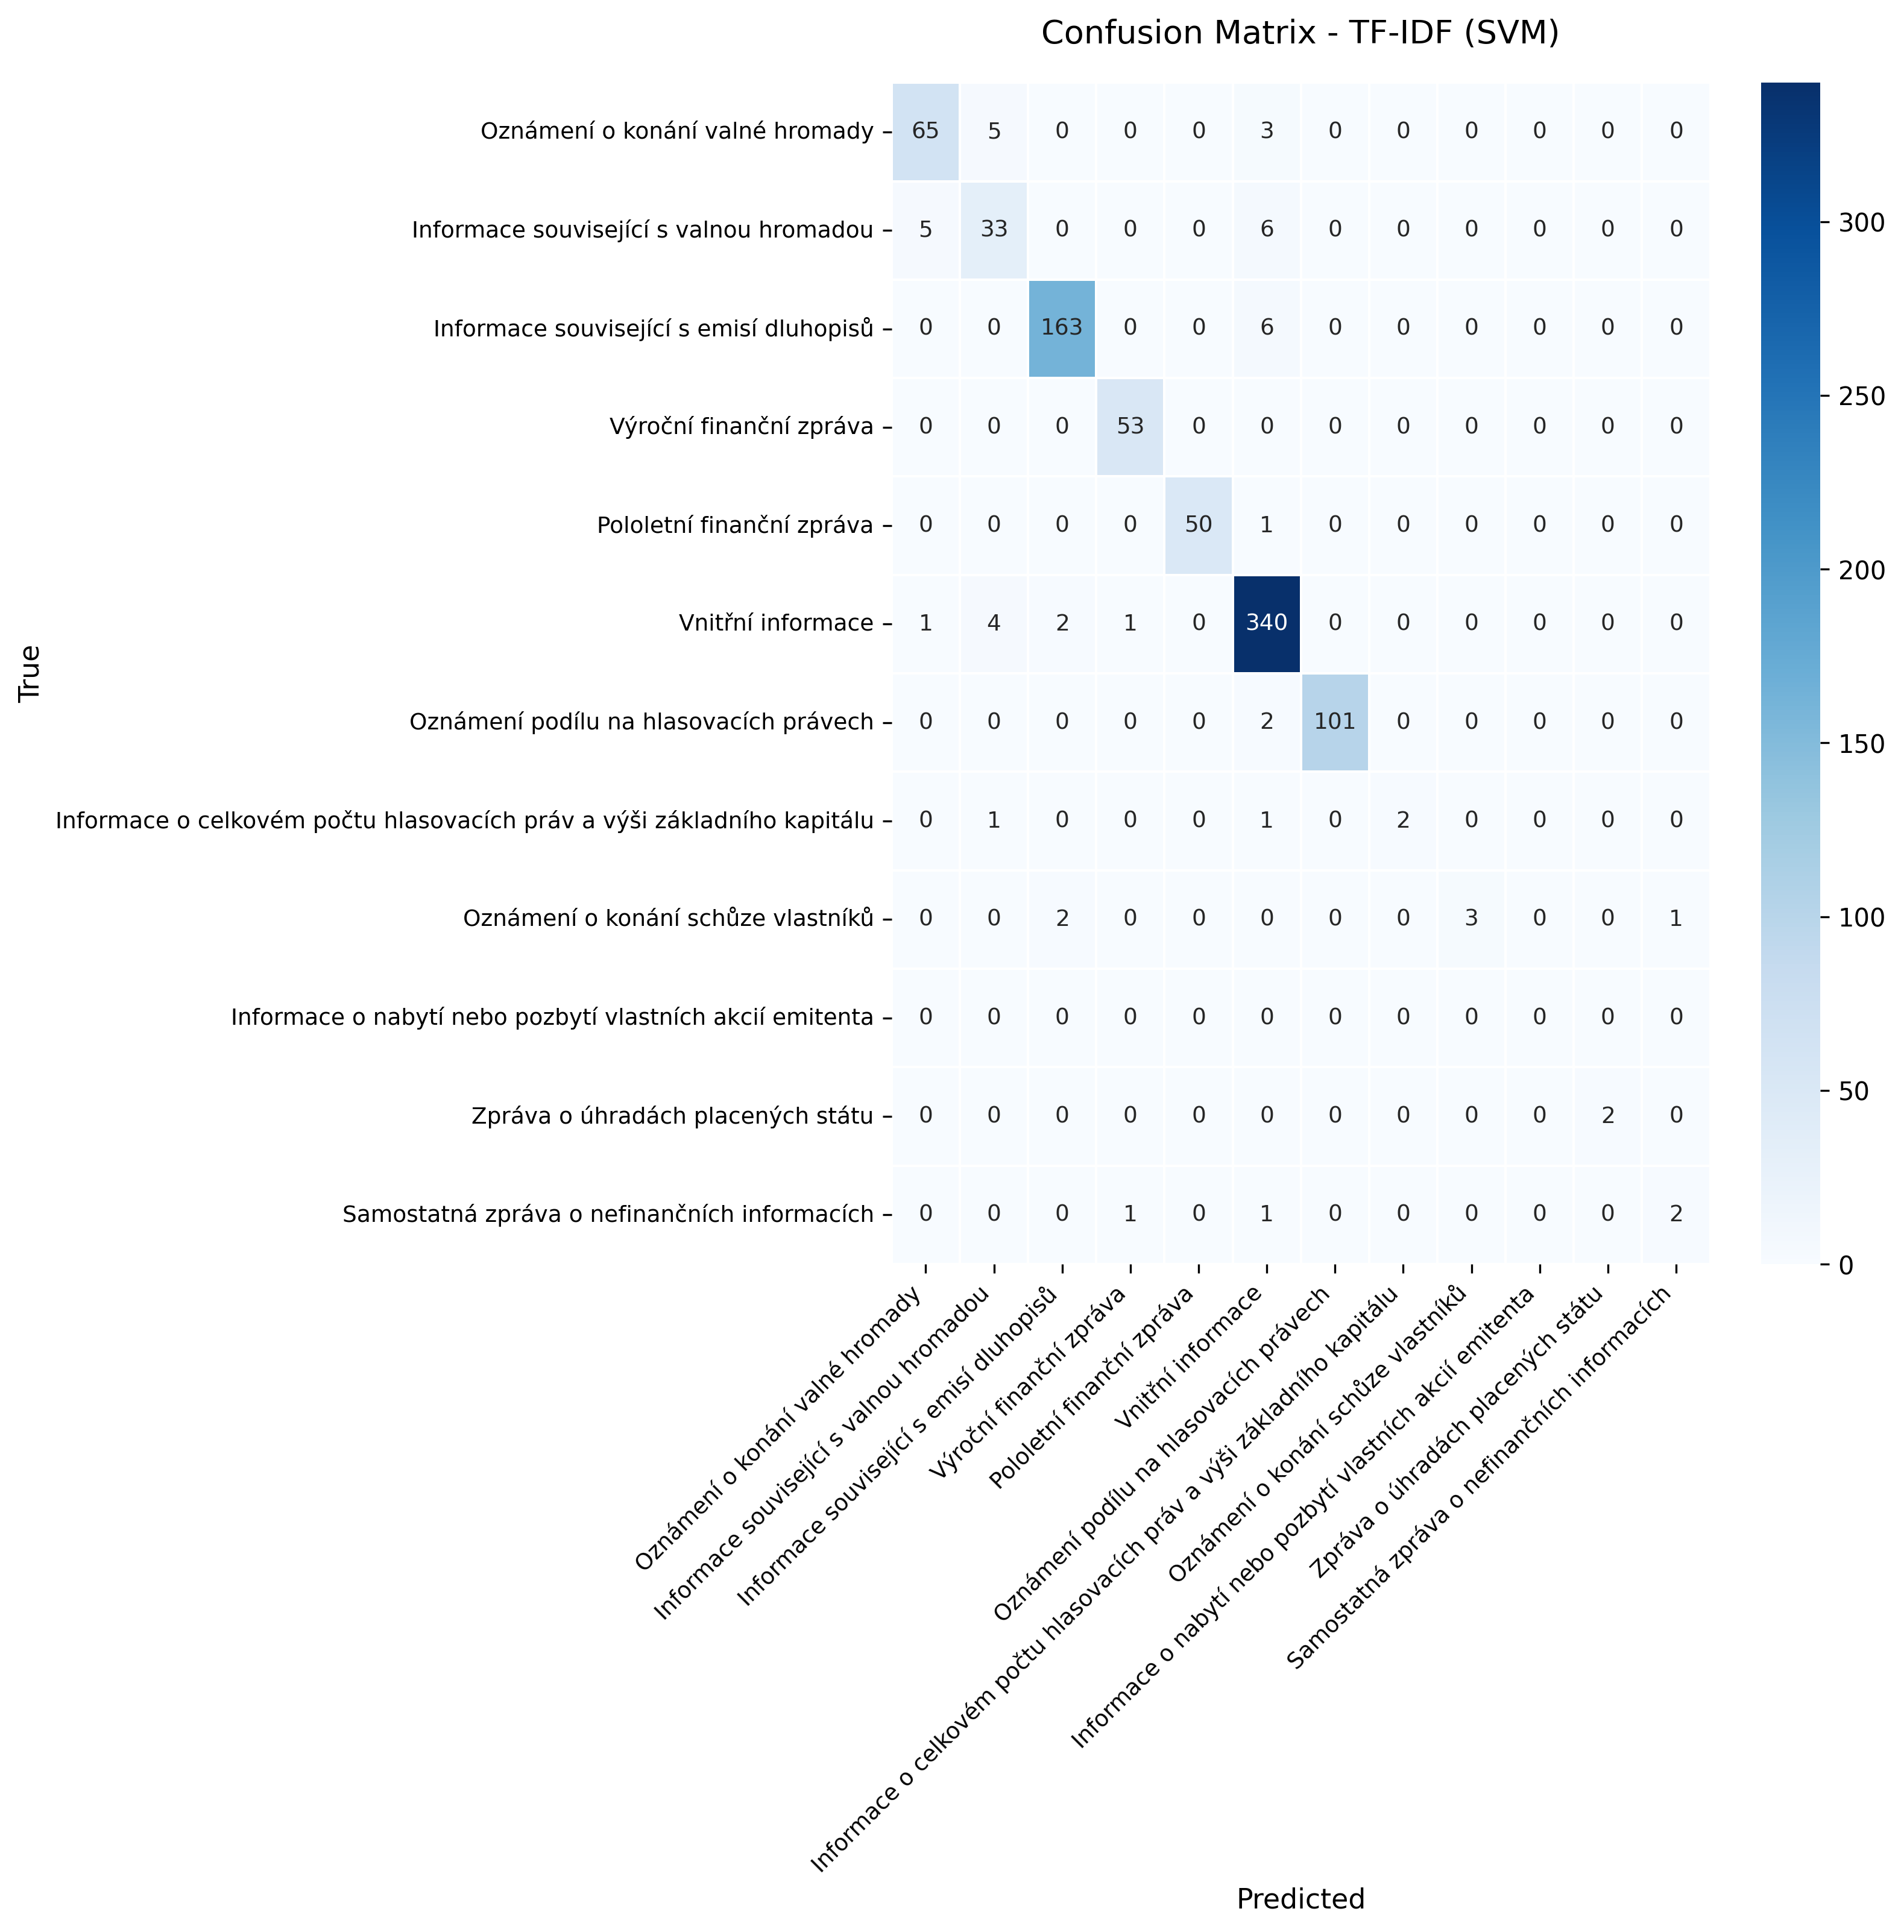
\includegraphics[width=0.85\textwidth]{img/confusion_matrix_tf-idf_svm.png}
    \caption{Matice záměn pro nejlepší model (TF-IDF + Linear SVM)}
    \label{fig:confusion_svm}
\end{figure}

% _____________________________________________________________________________
%        KAPITOLA 5: Závěr
% _____________________________________________________________________________
\chapter{Závěr}
V rámci této výzkumné zprávy jsme úspěšně navrhli, naimplementovali a vyhodnotili systém pro klasifikaci a validaci dokumentů regulovaných informací z portálu ČNB OAM. Vyřešili jsme technické problémy s dynamickým scrapingem a paginací pomocí date-range krájení a dynamic iframe waitů. 

V klasifikační úloze se jako nejúspěšnější ukázal model TF-IDF ve spojení s lineárním SVM, který dosáhl přesnosti 95,0~\%. Tradiční supervised modely výrazně předčily zero-shot nasazení velkého jazykového modelu Gemma 3 (12B) běžícího na univerzitním serveru, který na rozšířeném datasetu 12 kategorií dosáhl přesnosti 66,3~\% bez nutnosti lokálního dotrénování. 

Pro produkční nasazení doporučujeme hybridní přístup:
\begin{itemize}
    \item Použití lehkého lokálního SVM modelu pro rychlou předběžnou kontrolu dokumentů přímo v klientské aplikaci.
    \item Využití Gemma 3 LLM modelu pro detailnější audit a generování textových zdůvodnění v češtině u dokumentů, kde SVM vykazuje nízké skóre spolehlivosti (mismatch/warning).
\end{itemize}

V budoucí práci plánujeme rozšířit projekt o fine-tuning menšího lokálního transformátorového modelu (např. RobeCzech) pomocí připraveného Jupyter zápisníku v Google Colab a otestovat pokročilejší metody extrakce textu ze skenovaných PDF dokumentů pomocí OCR knihoven.

\backmatter
\nocite{*}
\printbibliography
\backpage
\end{document}
